\documentclass[12pt]{article}

\usepackage{sbc-template}
\usepackage{graphicx,url}
\graphicspath{{images/}}

\usepackage[brazil]{babel}
\usepackage[latin1]{inputenc}

\usepackage[alf,bibjustif,abnt-full-initials=no,abnt-etal-cite=2,abnt-and-type=1,abnt-etal-text=it,abnt-url-package=url,abnt-emphasize=bf]{abntcite}%[alf]{abntcite}

\usepackage{float}
\usepackage{subfigure}
\usepackage{setspace}

\sloppy

\title{Comparativo de protocolos de roteamento em redes \textit{ad hoc} m\'oveis em cen\'arios militares.}
\author{
	F\'abio Leandro Janiszevski\inst{1}, 
	Dr. Daniel Kikuti\inst{1}, 
	Ms. Hermano Pereira\inst{2}
}
\address{
	Universidade Estadual do Centro-Oeste - UNICENTRO
\nextinstitute
	Universidade Tecnol\'ogica Federal do Paran\'a - UTFPR
\email{
	fabiosammy@gmail.com,
	danielkikuti@yahoo.com.br,
	hermanopereira@utfpr.edu.br}
}

\pagestyle{myheadings}
\markright{}  % para book, report articles

\begin{document}
  \setlength{\leftmargini}{1.70cm}
  \setlength{\labelsep}{.5em}
  \setlength{\parindent}{1.27cm}
  \setlength{\parskip}{6pt}

\maketitle

\begin{abstract}
This article presents a study of different routing protocols in ad hoc networks, analyzing the performance in military scenarios, making comparisons between them through simulations with the NS-2 tool.
Where we used the protocols DSDV, and OLSR AODL in 2 different scenarios, of which we can analyze the performance a little of each.
\end{abstract}

\begin{keyWord}
Ad hoc networks; military scenarios, routing protocols, AODV, DSDV, OLSR;
\end{keyWord}

\begin{resumo}
Este artigo apresenta um estudo de diferentes protocolos de roteamento em redes ad hoc, analizando a performance em cen\'arios militares, realizando compara\c{c}\~oes entre os mesmos atrav\'es de simula\c{c}\~oes com a ferramenta NS-2. 
Onde foram utilizados os protocolos DSDV, AODL e OLSR em 2 diferentes cen\'arios, dos quais podemos analizar um pouco o desempenho de cada um.
\end{resumo}

\begin{palavraChave}
Redes ad hoc; Cen\'arios militares; Protocolos de roteamento; AODV; DSDV; OLSR;
\end{palavraChave}

%configurações gerais
\singlespacing

\section{Introdu\c{c}\~ao} 

Atualmente a maioria da popula\c{c}\~ao possui um dispositivo port\'atil com disponibilidade de conex\~ao a redes sem-fio e capaz de se comunicar com outros dispositivos. Com a populariza\c{c}\~ao destes dispositivos, \'e muito comum existirem in\'umeras redes sem-fio dispon\'iveis para conex\~ao abertamente, ou a possibilidade de se criar uma nova conforme necessidade.

As redes sem-fio s\~ao chamadas de wireless, elas provem comunica\c{c}\~ao, seja com uma pequena ou grande rede de comunica\c{c}\~ao. Nesse tipo de comunica\c{c}\~ao existem 2 divis\~oes redes infra-estruturadas e redes ad hoc. As redes ad hoc s\~ao consideradas m\'oveis(MANETs), pois n\~ao \'e necess\'ario uma estrutura fixa para que a comunica\c{c}\~ao funcione.

\begin{quote}
As redes m\'oveis sem-fio podem ser classificadas de duas formas: redes infra-estruradas e redes ad hoc. Nas redes infra-estruturadas, toda a comunicac\~ao entre os n\'os m\'oveis \'e feita por meio de esta\c{c}\~oes de suporte \`a mobilidade na rede fixa. Neste tipo de rede, os n\'os m\'oveis, mesmo pr\'oximos um do outro, est\~ao impossibilitados de estabelecer comunica\c{c}\~ao direta entre si.
\end{quote}

\begin{quote}
As MANETs proporcionam a exist\^encia de estruturas de comunica\c{c}\~ao em ambientes, por exemplo, com muitos obst\'aculos \`a cria\c{c}\~ao de uma estrutura fixa. Um cen\'ario de opera\c{c}\~ao militar pode ser visto como uma situa\c{c}\~ao em que as MANETs s\~ao requiridas para proporcionar a comunica\c{c}\~ao em um ambiente hostil e geograficamente acidentado, n\~ao possibilitando a exist\^encia de uma estrutura fixa.\cite{brignoni}
\end{quote}

Conforme \cite{pepe} comentam sobre a dinamicidade das redes ad hoc e a facilidade em criar uma rede nesse tipo, um cen\'ario militar \'e uma \'otima aplicacao desse tipo de rede, pois tal cen\'ario \'e um ambiente hostil e geograficamente acidentado, n\~ao possibilitando a exist\^encia de uma estrutura fixa \cite{schimidt}.

Segundo \cite{salles}, a necessidade de uma comunica\c{c}\~ao r\'apida para a equipe militar \'e essencial para obter um sucesso em sua operac\~ao, pois qualquer atraso na comunicac\~ao pode influenciar em um final catastr\'ofico na execuc\~ao de um passo na operac\~ao. Os diversos protocolos existentes das redes ad hoc diferenciam-se em n\'umero de pacotes de requisic\~oes a transitar na rede, modo de atualizac\~ao das rotas, sistema de armazenamento de rotas, e outros. o que influencia na performance final da rede.
		%Introdução
%\section{Hist\'orico}

		%Histórico
\section{Protocolos de roteamento em redes \textit{ad hoc}}\label{protocols}

Em redes m\'oveis \textit{ad hoc}, uma rota entre dois n\'os pode ser formada por saltos atrav\'es de um ou mais n\'os na rede, na qual, cada salto representa uma passagem por diferentes n\'os at\'e chegar ao destino desejado. 

Os protocolos de roteamento em redes \textit{ad hoc} precisam trabalhar, constantemente, com as trocas de topologia da rede, a qual acarreta em atualizar ou procurar novas rotas entre os n\'os da rede. 
A troca de topologia ocorre quando um n\'o da rede se desloca fisicamente na \'area de comunica\c{c}\~ao, alterando a conex\~ao com os vizinhos, e encontra novas ou perde antigas conex\~oes.

Os protocolos de roteamento s\~ao variados, mas segundo \cite{gorantala}, somente dois s\~ao de suma import\^ancia nas redes \textit{ad hoc}, sendo o DSDV(\textit{Destination Sequenced Distance Vector}), para redes pequenas, e o AODV(\textit{Ad-hoc On-Demand Distance Vector}), para redes \textit{ad hoc} em geral. 
Cada protocolo trabalha de forma diferente, podendo ser pr\'o-ativo ou reativo. 
"Os protocolos pr\'o-ativos mant\^em rotas para todos os n\'os da rede, independente do uso ou necessidade destas rotas. (...) J\'a os protocolos reativos iniciam as atividades de roteamento de acordo com a demanda" \cite{pereira}.

Os protocolos de roteamento estudados s\~ao baseados em dois tipos de algoritmos, em Vetor de Dist\^ancia, ou em Estado de Enlace. 
Os protocolos baseados em Vetor de Dist\^ancia possuem as tabelas de roteamento atualizadas atrav\'es da troca de mensagens com seus vizinhos, e mant\'em apenas as melhores rotas nesta tabela. 
Em intervalos de tempos regulares, as tabelas de roteamento s\~ao enviadas apenas para seus vizinhos, que por sua vez, atualizam suas tabelas. 
E o protocolo de roteamento que \'e baseado em Estado de Enlace tamb\'em possui as tabelas de roteamento atualizadas atrav\'es da troca de mensagens com seus vizinhos, por\'em, mant\'em todas as informa\c{c}\~oes de conex\~oes da rede na tabela. 
O pr\'oprio protocolo descobre o melhor caminho, pois a rota possui o identificador de interface, n\'umero de enlace e m\'etrica. 
No momento em que ocorre uma altera\c{c}\~ao no estado de enlace da rede, os n\'os adjacentes percebem e notificam os vizinhos, que por sua vez, atualizam a rota se ela for nova \cite{posselt}.

Os roteadores em uma rede \textit{ad hoc} trocam informa\c{c}\~oes de roteamento uns com os outros, com a finalidade de tomar conhecimento das disponibilidades de rotas e da topologia da rede \cite{pereira}. 
Essa troca de informa\c{c}\~oes pode acarretar em \textit{loop} de roteamento, o qual \'e uma condi\c{c}\~ao em que um pacote \'e transmitido continuamente em uma s\'erie de n\'os, sem sequer alcan\c{c}ar seu n\'o de destino desejado. 
Esse \textit{loop} pode ocorrer quando dois ou mais n\'os t\^em informa\c{c}\~oes de roteamento que indicam, de forma incorreta, que uma rota \'e v\'alida para um n\'o de destino. Por\'em, esse n\'o de destino \'e inalcan\c{c}\'avel atrav\'es desta mesma rota. 
Essa \'e mais uma condi\c{c}\~ao em que os protocolos de roteamento precisam trabalhar e corrigir \cite{hengartnet}.

As subse\c{c}\~oes \ref{subDSDV}, \ref{subAODV} e \ref{subOLSR} apresentam os protocolos DSDV, AODV e OLSR, respectivamente, os quais s\~ao analisados nos experimentos desse trabalho.

\subsection{\textit{Destination sequenced distance vector} - DSDV} 
O protocolo DSDV \'e um protocolo de roteamento proativo\cite{gorantala}, baseado no algoritmo de vetor de dist\^ancias, que trabalha requisitando periodicamente, de cada um dos n\'os vizinhos, suas tabelas de roteamento, com a finalidade de mant\^e-las atualizadas. 
Cada n\'o da rede mant\'em uma tabela de roteamento, contendo o pr\'oximo salto e o n\'umero de saltos para cada destino alcan\c{c}\'avel. 
As tabelas incluem rotas para todos os n\'os da rede, mesmo que nunca seja necess\'ario enviar pacote para este n\'o. 
Cada n\'o mant\'em apenas uma rota para cada destino.

Os \textit{loops} de rotas podem ocorrer quando informa\c{c}\~oes de roteamento incorretas s\~ao mantidas na rede ap\'os uma troca de topologia. 
Geralmente, ocorre quando um n\'o detecta uma queda no enlace com o n\'o vizinho e, antes que consiga propagar sua nova tabela, recebe de outro n\'o informa\c{c}\~ao desatualizada referente \`a conex\~ao interrompida. 
A vantagem principal do DSDV sobre os protocolos baseados em vetor de dist\^ancias tradicionais \'e que ele garante a aus\^encia de \textit{loops}, usando o conceito de n\'umero de sequ\^encia mantido em cada rota. 
O n\'umero de sequ\^encia \'e estabelecido pelo n\'o destino e \'e incrementado a cada novo aviso de rota.
As rotas mais recentes possuem um n\'umero de sequ\^encia maior e s\~ao as mais favor\'aveis. 
Caso os n\'umeros de sequ\^encia sejam iguais, a rota que tiver o menor n\'umero de saltos ser\'a a mais favor\'avel. 
Neste contexto, o uso de n\'umeros de sequ\^encia faz com que o DSDV se adapte melhor para redes de topologia din\^amica como redes \textit{ad hoc}.

\subsubsection{Exemplo de funcionamento do DSDV}

A Figura \ref{figOpDSDV}, descreve uma rede com 8 hosts. 
Podemos analisar a mudan\c{c}a de roteamento da tabela do MH4 em rela\c{c}\~ao ao movimento do \textit{host} MH1(\textit{Mobile Host} 1), onde o movimento \'e representado pelas setas com estilo pontilhado. 

\begin{figure}[H]
	\centering
	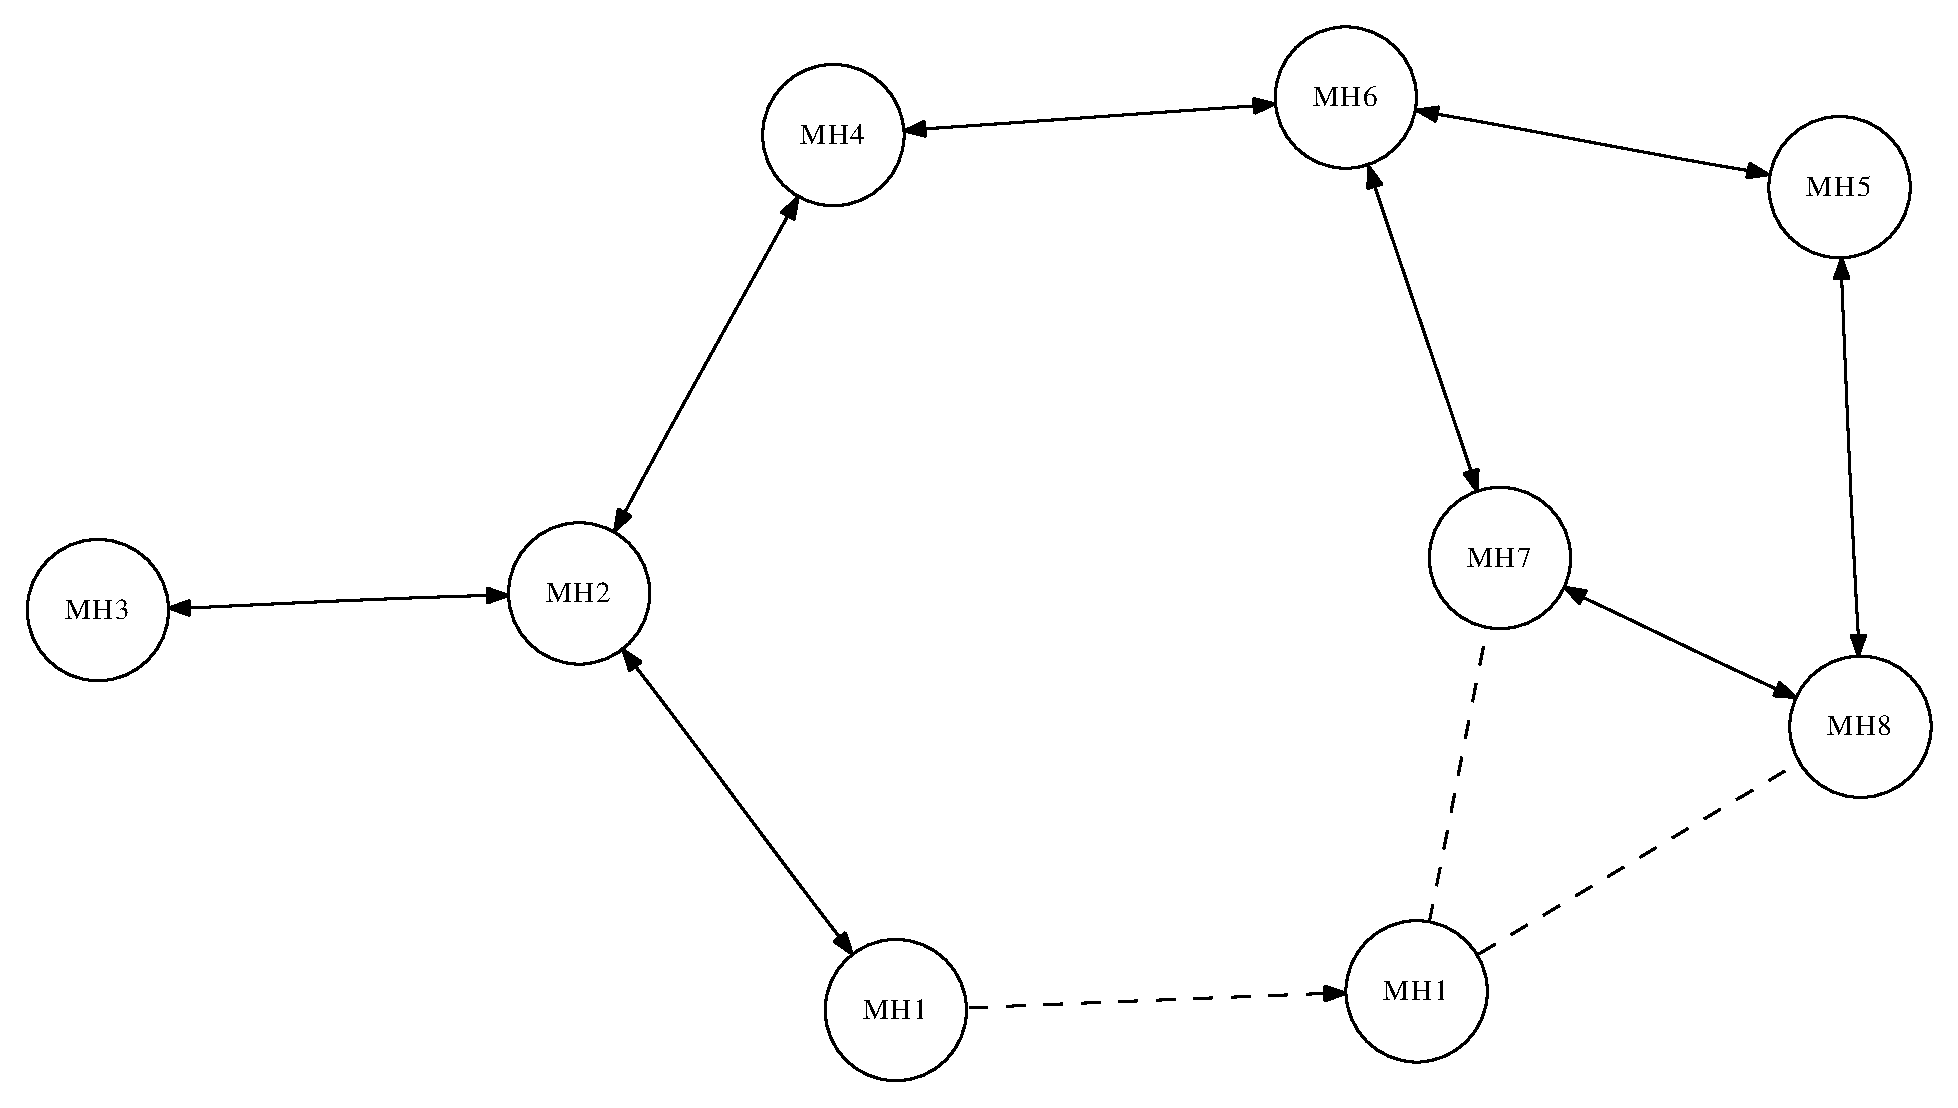
\includegraphics[scale=.4]{dsdvOperation.eps}
	\caption{Exemplo de opera\c{c}\~ ao do DSDV}
	\label{figOpDSDV}
\end{figure}

Uma tabela de roteamento do DSDV, cont\'em, para cada n\'o na rede:
\begin{itemize}
	\item Informa\c{c}\~oes do n\'o de destino;
	\item o pr\'oximo salto na rota para alcan\c{c}ar o destino;
	\item a m\'etrica com o valor de quantos saltos s\~ao necess\'arios para alcan\c{c}ar o destino;
	\item o n\'umero de sequ\^encia utilizado para sincroniza\c{c}\~ao das rotas;
	\item o install, atuando como um marcador de tempo da rota, para decidir de deletar ou n\~ao uma nova informa\c{c}\~ao topol\'ogica; e
	\item o campo informa\c{c}\~ao, servindo como um ponteiro para indicar a tabela com informa\c{c}\~oes sobre a estabilidade da rota.
\end{itemize}

Inicialmente, todos os n\'os anunciam suas informa\c{c}\~oes de roteamento para todos os outros n\'os da rede e, portanto, onde a tabela de roteamento do \textit{host} MH4 inicialmente apresenta o seguinte conte\'udo conforme a tabela \ref{tabRtMH4}.

\begin{table}[H]
	\centering
	\caption{Tabela de roteamento do \textit{host} MH4 \cite{pebha}}
	\begin{tabular}{ | c | c | c | c | c | c | }
		\hline
		Destino & Pr\'oximo salto & M\'etrica & N\'umero de sequ\^encia & Install & Informa\c{c}\~ao \\ \hline
		MH1 & MH2 & 2 & S406\_MH1 & T001\_MH4 & Ptr1\_MH1 \\ \hline
		MH2 & MH2 & 1 & S128\_MH2 & T001\_MH4 & Ptr1\_MH2 \\ \hline
		MH3 & MH2 & 2 & S564\_MH3 & T001\_MH4 & Ptr1\_MH3 \\ \hline
		MH4 & MH4 & 0 & S710\_MH4 & T001\_MH4 & Ptr1\_MH4 \\ \hline
		MH5 & MH6 & 2 & S309\_MH5 & T002\_MH4 & Ptr1\_MH5 \\ \hline
		MH6 & MH6 & 1 & S076\_MH6 & T001\_MH4 & Ptr1\_MH6 \\ \hline
		MH7 & MH6 & 2 & S128\_MH7 & T002\_MH4 & Ptr1\_MH7 \\ \hline
		MH8 & MH6 & 3 & S050\_MH8 & T002\_MH4 & Ptr1\_MH8 \\ \hline
	\end{tabular}
	\label{tabRtMH4}
\end{table}

Por\'em, quando o \textit{host} MH1 move sua localiza\c{c}\~ao para pr\'oximo dos \textit{hosts} MH7 e MH8 como apresentado na Figura \ref{figOpDSDV} ent\~ao, o enlace entre MH2 e MH1 vai ser quebrado, resultando em atribui\c{c}\~ao de uma m\'etrica infinita de MH2 para MH1 e o n\'umero de sequ\^encia ser\'a alterado para um n\'umero \'impar na tabela de roteamento em MH2. 
MH2 atualizar\'a essa informa\c{c}\~ao para os \textit{hosts} vizinhos. 
Desde que haja um novo \textit{host} vizinho para MH7 e MH8, eles v\~ao atualizar essa informa\c{c}\~ao nas respectivas tabelas de roteamento e propagar essa nova informa\c{c}\~ao. 
Agora, MH4 receber\'a esta atualiza\c{c}\~ao de informa\c{c}\~ao de MH6, onde MH6 recebe 2 pacotes de informa\c{c}\~oes de diferentes vizinhos para chegar em MH1 com o mesmo n\'umero de sequ\^encia, mas com diferentes m\'etricas. 
A sele\c{c}\~ao da rota ir\'a depender da menor contagem de saltos quando o n\'umero de sequ\^encia \'e o mesmo. 
Agora a tabela de roteamento do MH4 estar\'a com o conte\'udo demonstrado na tabela  \ref{tabNewRtMH4}.

\begin{table}[H]
	\centering
	\caption{Tabela de roteamento do \textit{host} MH4 depois do movimento do \textit{host} MH1 \cite{pebha}}
	\begin{tabular}{ | c | c | c | c | c | c | }
		\hline
		Destino & Pr\'oximo salto & M\'etrica & N\'umero de sequ\^encia & Install & Informa\c{c}\~ao \\ \hline
		MH1 & MH6 & 3 & S516\_MH1 & T001\_MH4 & Ptr1\_MH1 \\ \hline
		MH2 & MH2 & 1 & S238\_MH2 & T001\_MH4 & Ptr1\_MH2 \\ \hline
		MH3 & MH2 & 2 & S674\_MH3 & T001\_MH4 & Ptr1\_MH3 \\ \hline
		MH4 & MH4 & 0 & S820\_MH4 & T001\_MH4 & Ptr1\_MH4 \\ \hline
		MH5 & MH6 & 2 & S502\_MH5 & T002\_MH4 & Ptr1\_MH5 \\ \hline
		MH6 & MH6 & 1 & S186\_MH6 & T001\_MH4 & Ptr1\_MH6 \\ \hline
		MH7 & MH6 & 2 & S238\_MH7 & T002\_MH4 & Ptr1\_MH7 \\ \hline
		MH8 & MH6 & 3 & S160\_MH8 & T002\_MH4 & Ptr1\_MH8 \\ \hline
	\end{tabular}
	\label{tabNewRtMH4}
\end{table}

\subsubsection{Vantagens do DSDV}
\begin{itemize}
	\item Livre de \textit{loops} \cite{gorantala}.
	\item Problemas com contagem ao infinito \'e reduzido no DSDV \cite{gorantala}.
	\item Pode-se evitar tr\'afego extra com atualiza\c{c}\~oes incrementais, em vez de atualiza\c{c}\~oes de despejo completo.
	\item Sele\c{c}\~ao de caminho: O DSDV mant\'em somente o melhor caminho em vez de manter v\'arios caminhos para um mesmo destino. Com isso, o espa\c{c}o da tabela de roteamento \'e reduzido.
\end{itemize}

\subsubsection{Limita\c{c}\~ oes do DSDV}
\begin{itemize}
	\item Desperd\'icio do uso da banda na rede devido \`a propaga\c{c}\~ao desnecess\'aria de informa\c{c}\~oes de roteamento, mesmo se n\~ao houver mudan\c{c}as na topologia da rede \cite{Patel00energyin}.	
	\item O DSDV n\~ao suporta m\'ultiplos caminhos de rotas \cite{gorantala}.
	\item \'E dif\'icil determinar um tempo de converg\^encia para a propaga\c{c}\~ao das rotas \cite{heg}.
	\item \'E dif\'icil manter a propaga\c{c}\~ao das tabelas de rotas para uma grande rede. Cada \textit{host} na rede deve manter uma tabela de rotas para propaga\c{c}\~ao. Mas para uma grande rede, isso causaria \textit{overhead} de rede, o qual consome uma maior banda na rede \cite{gorantala}.
\end{itemize}
	%Destination sequenced distance vector - DSDV
\subsection{\textit{Ad hoc on demand distance vector} - AODV}\label{subAODV}
O protocolo AODV \'e um protocolo reativo\cite{gorantala}, baseado em Vetor de Dist\^ancias, e pode ser considerado como uma combina\c{c}\~ao de outros dois protocolos, denominados DSR e DSDV. 
O AODV tem a base do DSR, o qual \'e baseado na forma de trabalho sob demanda, ou seja, descobre rotas somente quando necess\'ario, e utiliza os mecanismos de descoberta de rotas e manuten\c{c}\~ao de rotas.
Entretanto, o AODV utiliza a caracter\'istica do DSDV de obrigar todos os n\'os intermedi\'arios a estabelecerem dinamicamente entradas em tabelas de roteamento locais para cada destino ativo.
Cada n\'o tem conhecimento do pr\'oximo salto para alcan\c{c}ar o destino e a dist\^ancia em n\'umero de saltos.
Pode ser considerado como uma vers\~ao melhorada do DSDV, uma vez que seu funcionamento baseado em demanda minimiza o n\'umero de inunda\c{c}\~oes na rede exigido pelo DSDV para cria\c{c}\~ao de rotas.

\subsubsection{Processo de descoberta de rotas no AODV}
Quando um n\'o necessita encontrar uma rota para outro n\'o, e esta rota n\~ao est\'a presente na sua tabela de rotas, inicia um procedimento de descoberta de rotas (Figura \ref{figAodvRreq}), enviando pacotes \textit{Route Request} (RREQ) para todos os n\'os vizinhos, incluindo o \'ultimo n\'umero de sequ\^encia para aquele destino. 
Os pacotes RREQ s\~ao propagados pela rede at\'e alcan\c{c}ar o n\'o destino ou um n\'o intermedi\'ario com uma rota recente para o destino.

\begin{figure}[H]
	\centering
	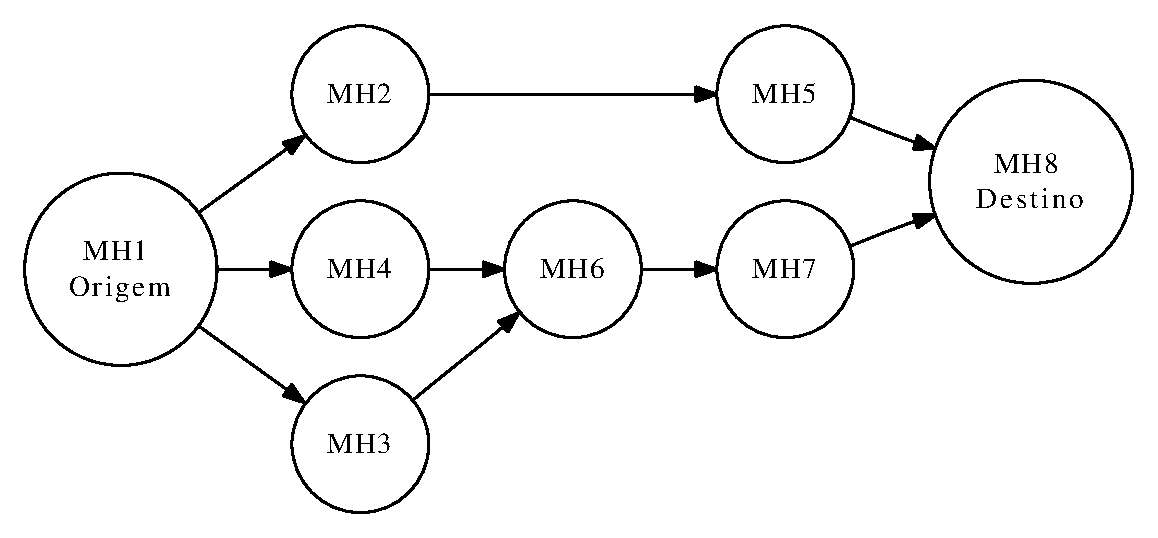
\includegraphics[scale=.5]{aodvRREQ.eps}
	\caption{Descoberta de rotas (RREQ) usando o protocolo AODV \cite{pereira}}
	\label{figAodvRreq}
\end{figure}

Durante o processo de encaminhamento do pacote RREQ, os n\'os intermedi\'arios gravam em suas tabelas de rotas o endere\c{c}o do vizinho que encaminhou o pacote. 
Desta forma, estabelece um caminho reverso que ser\'a utilizado pelo pacote \textit{Route Reply} (RREP) para alcan\c{c}ar o n\'o de origem (Figura \ref{figAodvRrep}), quando a rota para o destino for encontrada.

\begin{figure}[H]
	\centering
	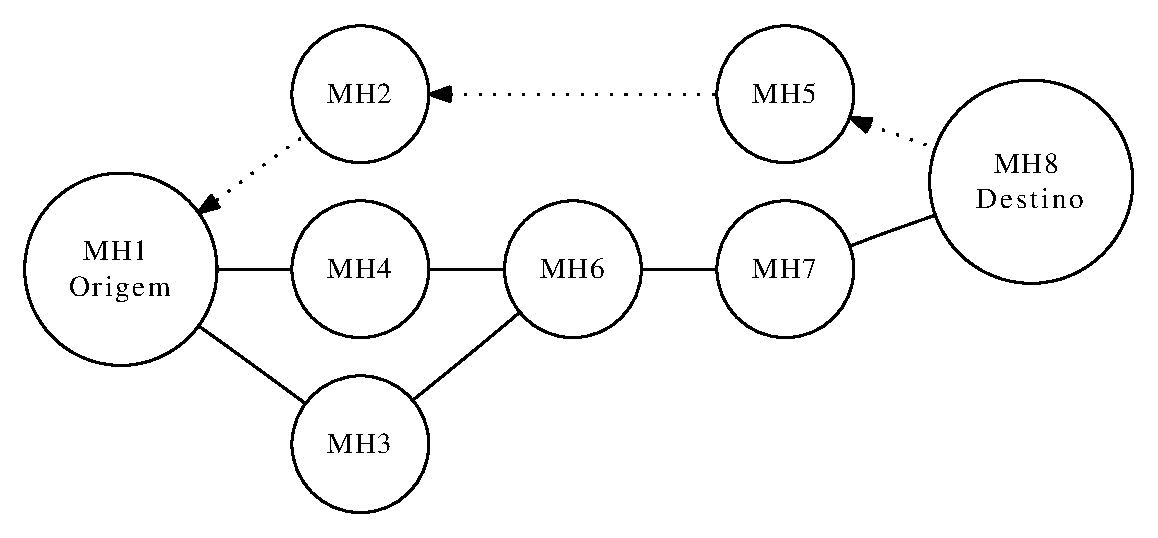
\includegraphics[scale=.5]{aodvRREP.eps}
	\caption{Propaga\c{c}\~ao do \textit{Route Reply} (RREP) no protocolo AODV \cite{pereira}}
	\label{figAodvRrep}
\end{figure}

Em cada tabela de roteamento \'e mantido o conjunto de n\'os antecessores que utilizam esta entrada para rotear pacotes de dados. Ent\~ao, quando uma conex\~ao \'e interrompida, estes n\'os antecessores s\~ao notificados com pacotes \textit{Route Error} (RERR). Cada n\'o antecessor encaminha este pacote para sua lista de n\'os antecessores, permitindo assim que efetivamente seja propagada a informa\c{c}\~ao de conex\~ao falha.

\begin{figure}[H]
	\centering
	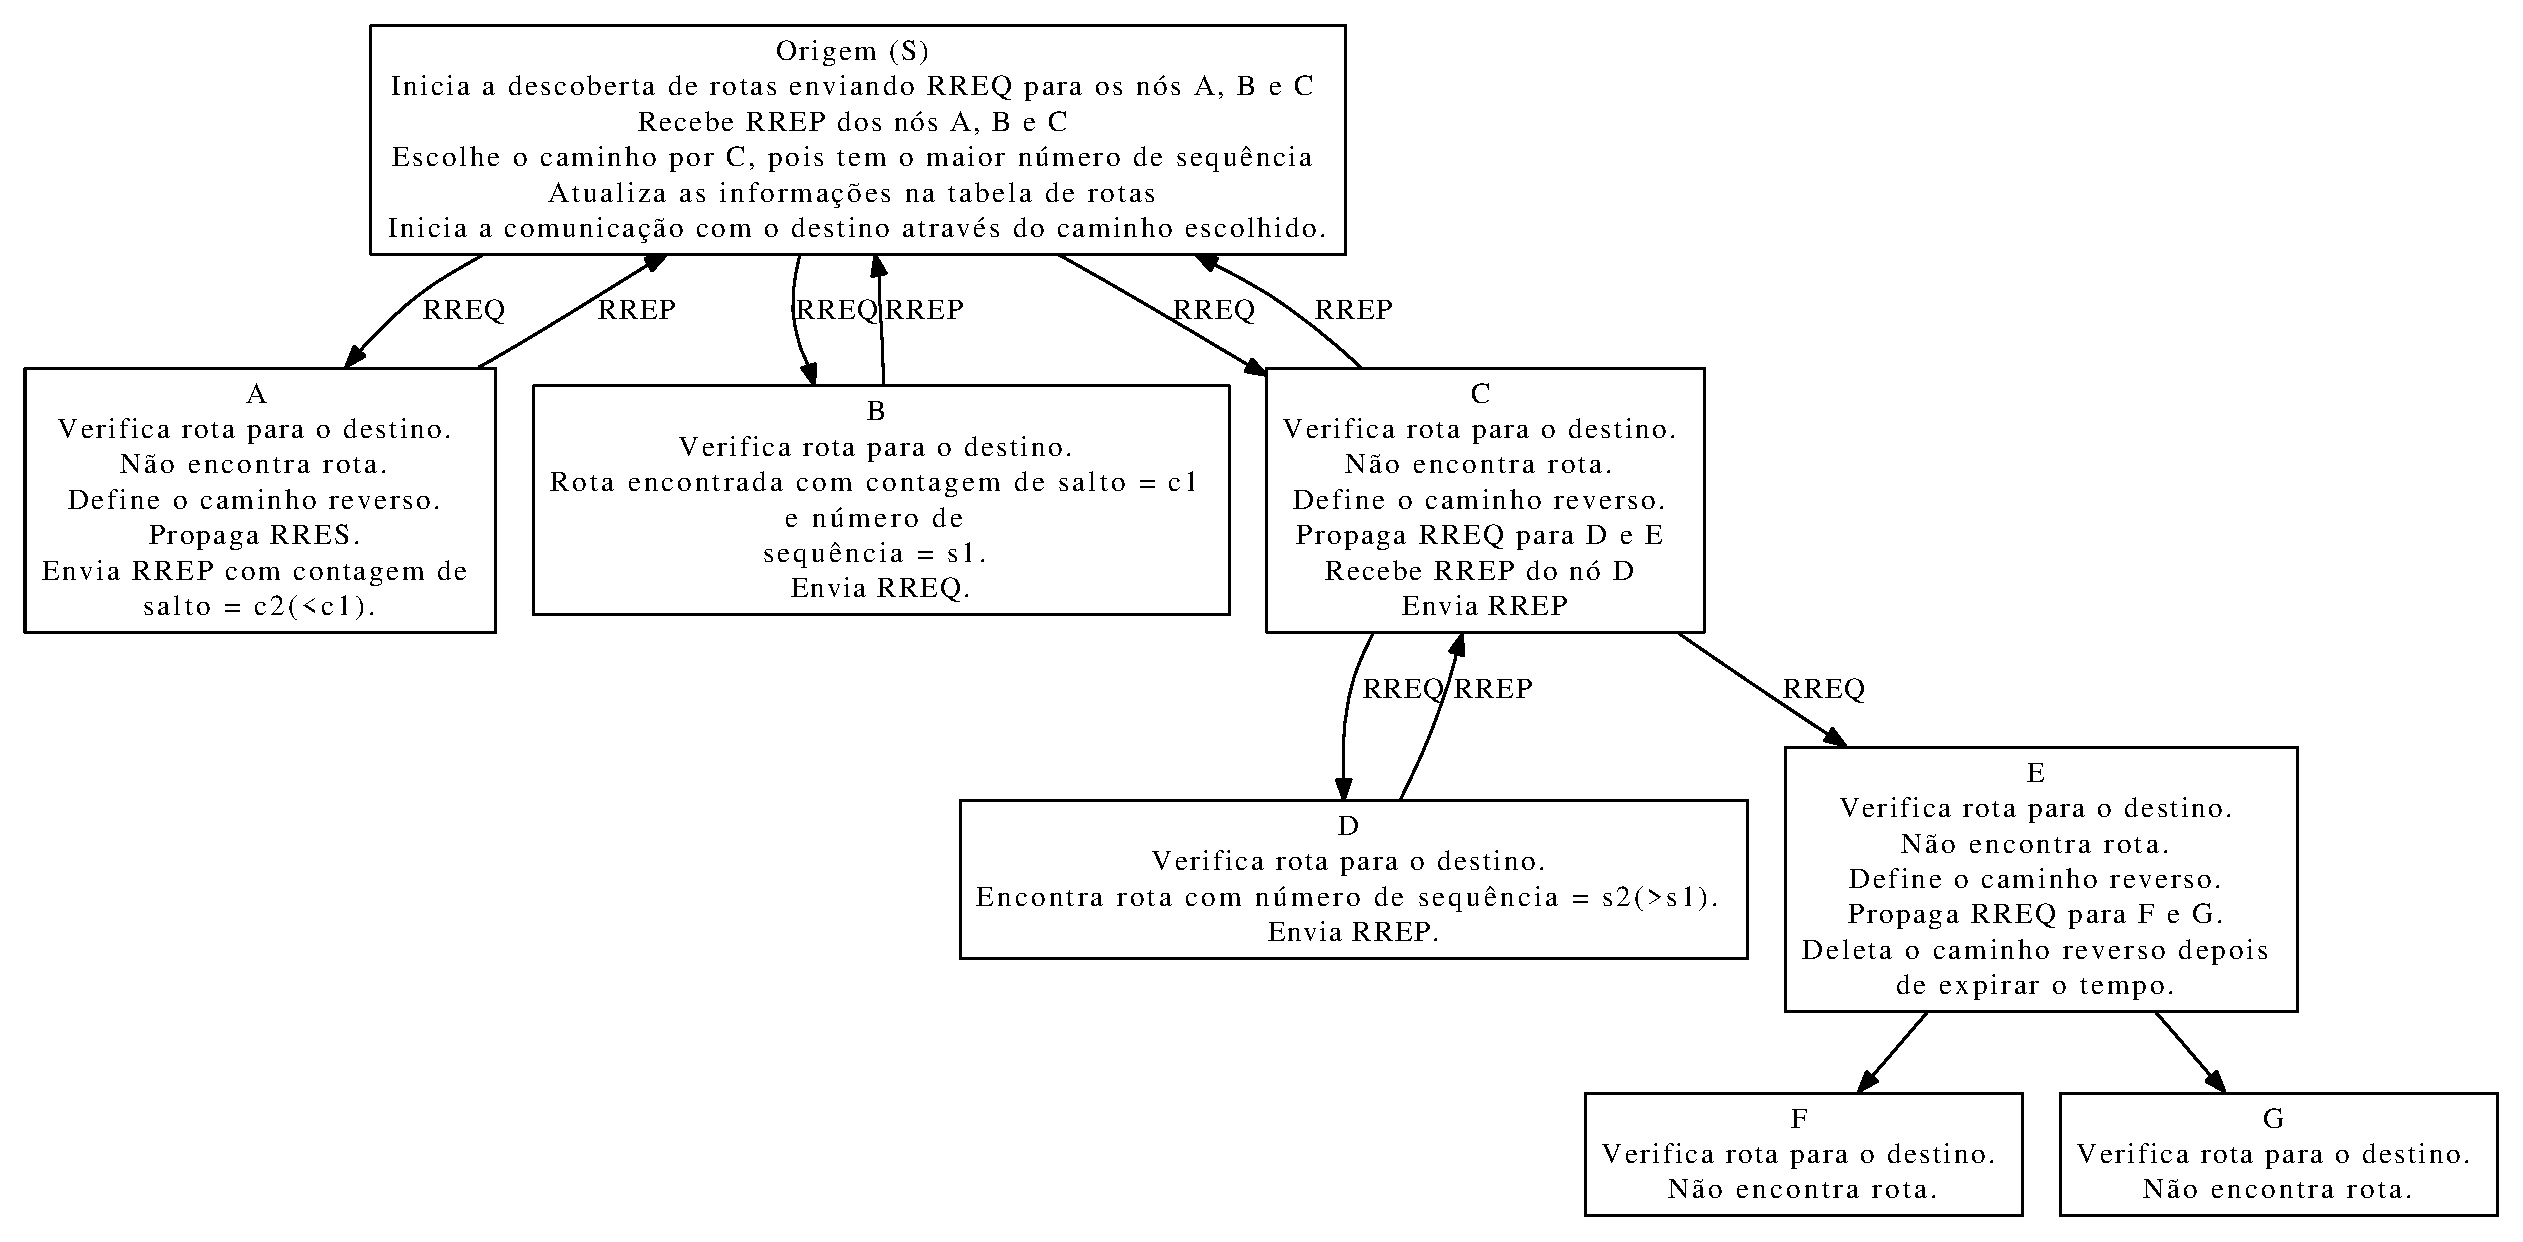
\includegraphics[scale=.43]{aodvOperation.eps}
	\caption{Processo de cria\c{c}\~ao de rotas no AODV \cite{gorantala}}
	\label{figOpAODV}
\end{figure}
Acima a Figura \ref{figOpAODV} \'e um exemplo de como o protocolo AODV encontra uma rota para um destino.
Segue passo-a-passo a explica\c{c}\~ao do processo exibido na Figura \ref{figOpAODV}:
\begin{enumerate}
	\item "Origem S" precisa enviar dados ao destino.
	\item "S" envia RREQ para seus vizinhos "A", "B" e "C".
	\item "B" encontra o caminho em sua tabela de roteamento (com n\'umero de sequ\^encia = s1 e contagem de salto = c1) e envia RREP para "S".
	\item "C" ativa caminho reverso.
	\item "C" redireciona RREQ para seus vizinhos "D" e "E".
	\item "E" ativa caminho reverso.
	\item "E" redireciona RREQ para seus vizinhos "F" e "G".
	\item "E" deleta o caminho reverso ap\'os um per\'iodo de tempo limite, uma vez que n\~ao recebe qualquer RREPs dos n\'os "F" e "G".
	\item "D" encontra o caminho para destn (com n\'umero de sequ\^encia = s2, o qual \'e maior que s1 e contagem de salto c1) em sua tabela de roteamento e envia RREP para "C".
	\item "C" recebe RREP de "D" e ativa o caminho de reencaminhamento e reencaminha RREP para "S".
	\item "A" define o caminho reverso; redireciona RREQ para seus vizinhos; recebe RREP (com caminho de contagem de saltos c2, o qual \'e maior que c1); define o caminho de redirecionamento; e redireciona o RREP para "S".
	\item "S" recebe uma inform\c{c}\~ao de caminho de "C" (o qual foi criado por "D"), dando prioridade ao caminho com o n\'umero de sequ\^encia maior e segunda prioridade com o caminho com a menor contagem de saltos. Apesar do caminho por "A" ter uma menor contagem de saltos, isso \'e ignorado, porque o n\'umero de sequ\^encia \'e maior para o caminho de "C".
\end{enumerate}

\subsubsection{Vantagens do AODV}
\begin{itemize}
	\item Por causa de sua natureza reativa, o AODV pode lidar com o comportamento din\^amico das redes \textit{ad hoc} \cite{schwingenschlogl}.
	\item Utilizado tanto para \textit{unicasts} quanto \textit{multicasts} com a \textit{flag} 'J'\footnote{\textit{Join in group} - Usado para aproveitar rota de outros n\'os.} nos pacotes \cite{ramachandranTech}.
\end{itemize}

\subsubsection{Limita\c{c}\~oes e desvantagens do AODV}
\begin{itemize}
	\item \textbf{Necessidade de um meio de propaga\c{c}\~ ao:} O algoritmo necessita que os n\'os no meio da propaga\c{c}\~ ao possam detectar outras propaga\c{c}\~oes \cite{gorantala}.
	\item \textbf{N\~ao reutiliza informa\c{c}\~oes de roteamento:} O AODV carece de efici\^encia na t\'ecnica de manuten\c{c}\~ao de suas rotas. Informa\c{c}\~oes de roteamento s\~ao sempre atualizadas em cada demanda, inclu\'indo casos comuns de tr\'afego \cite{ramachandran}.
	\item \textbf{O AODV n\~ao tem um suporte para altas demandas de roteamento:} O protocolo AODV foi destinado para suportar uma pequena contagem de saltos \cite{ramachandran}.
\end{itemize}
	%Ad hoc on demand distance vector} - AODV
\subsection{\textit{Optimized link state routing} - OLSR}
O protocolo OLSR \'e um protocolo pr\'o-ativo
Pr\'o-ativo, marca\c{c}\~ao especial dos vizinhos.

\begin{figure}[H]
	\centering
	\subfigure[Primeiro est\'agio]{
		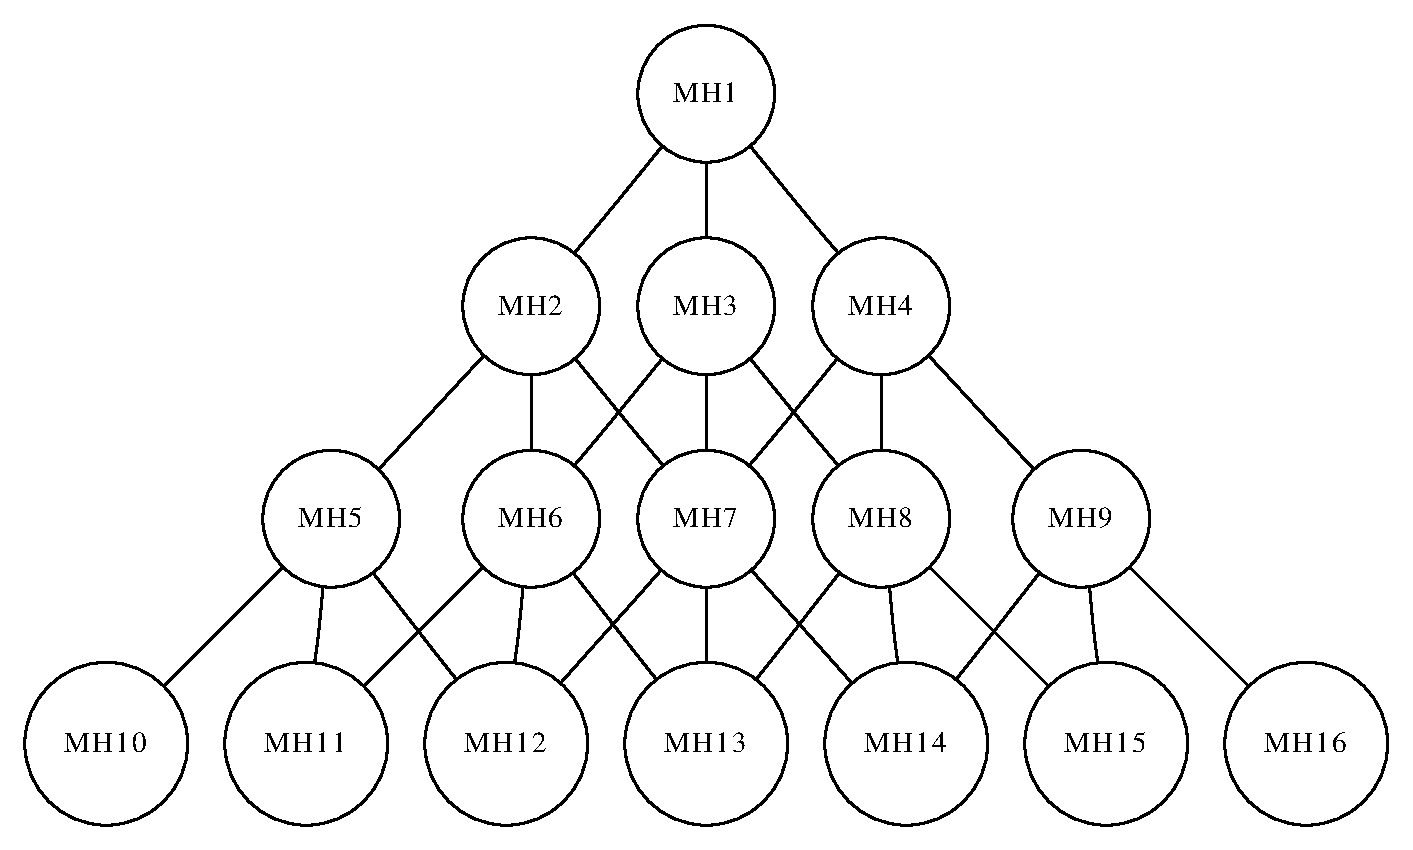
\includegraphics[scale=0.3]{olsrOperationStep1.eps}
	}\label{subfig:olsrStep11}
	\subfigure[Segundo est\'agio]{
		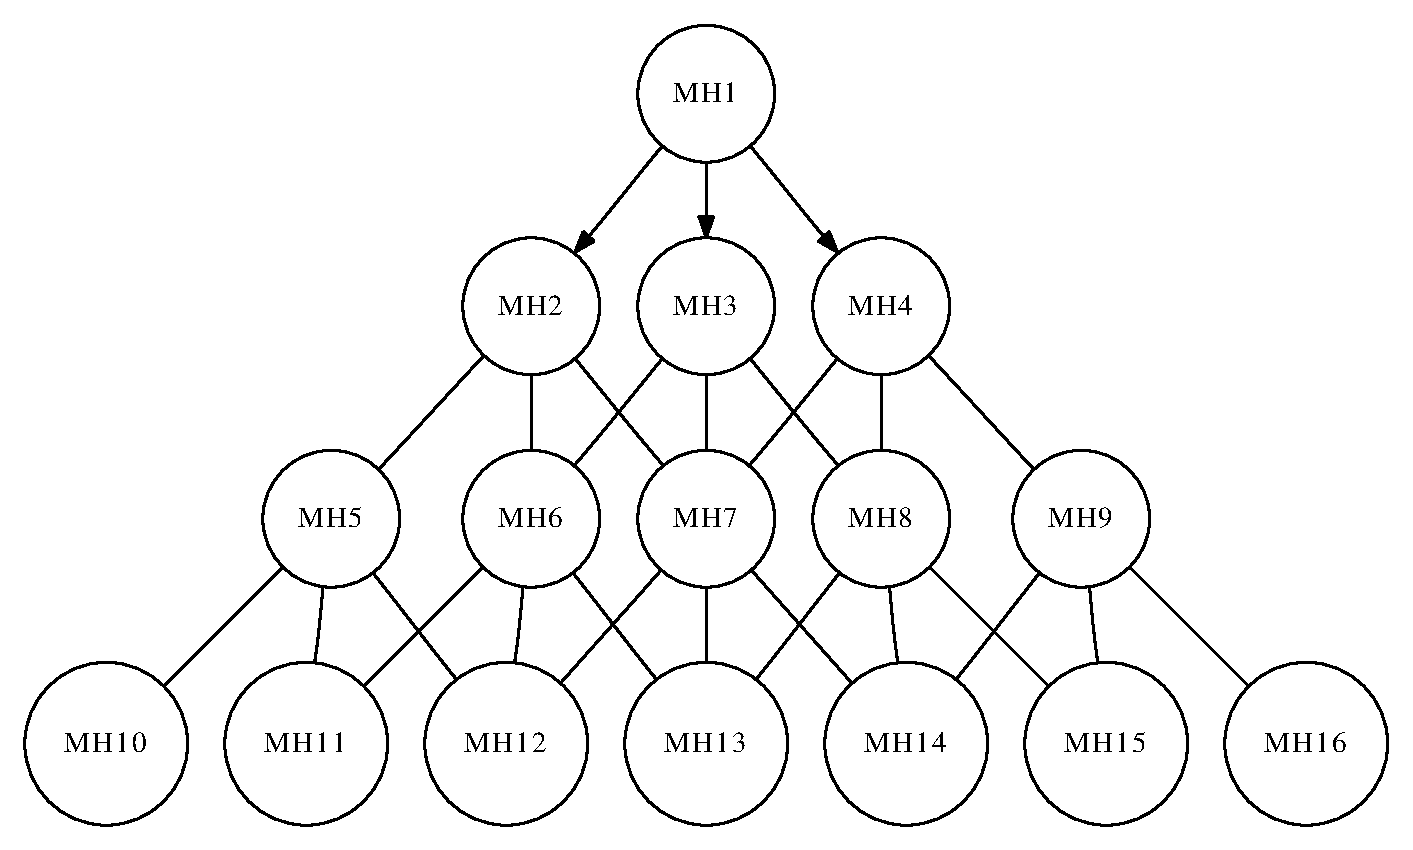
\includegraphics[scale=0.3]{olsrOperationStep2.eps}
	}\label{subfig:olsrStep12}
	\subfigure[Terceiro est\'agio]{
		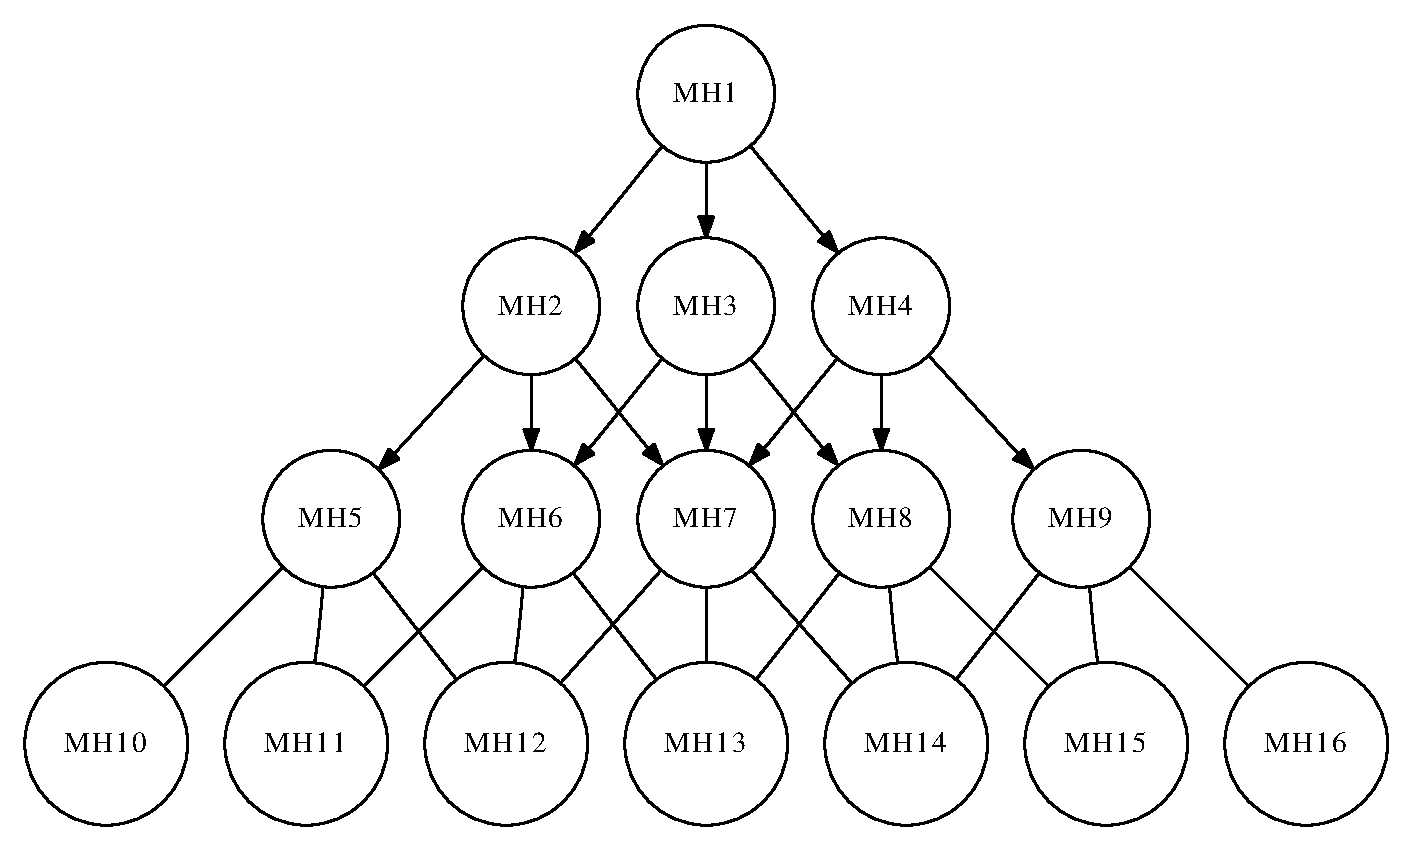
\includegraphics[scale=0.3]{olsrOperationStep3.eps}
	}\label{subfig:olsrStep13}
	\subfigure[Quarto est\'agio]{
		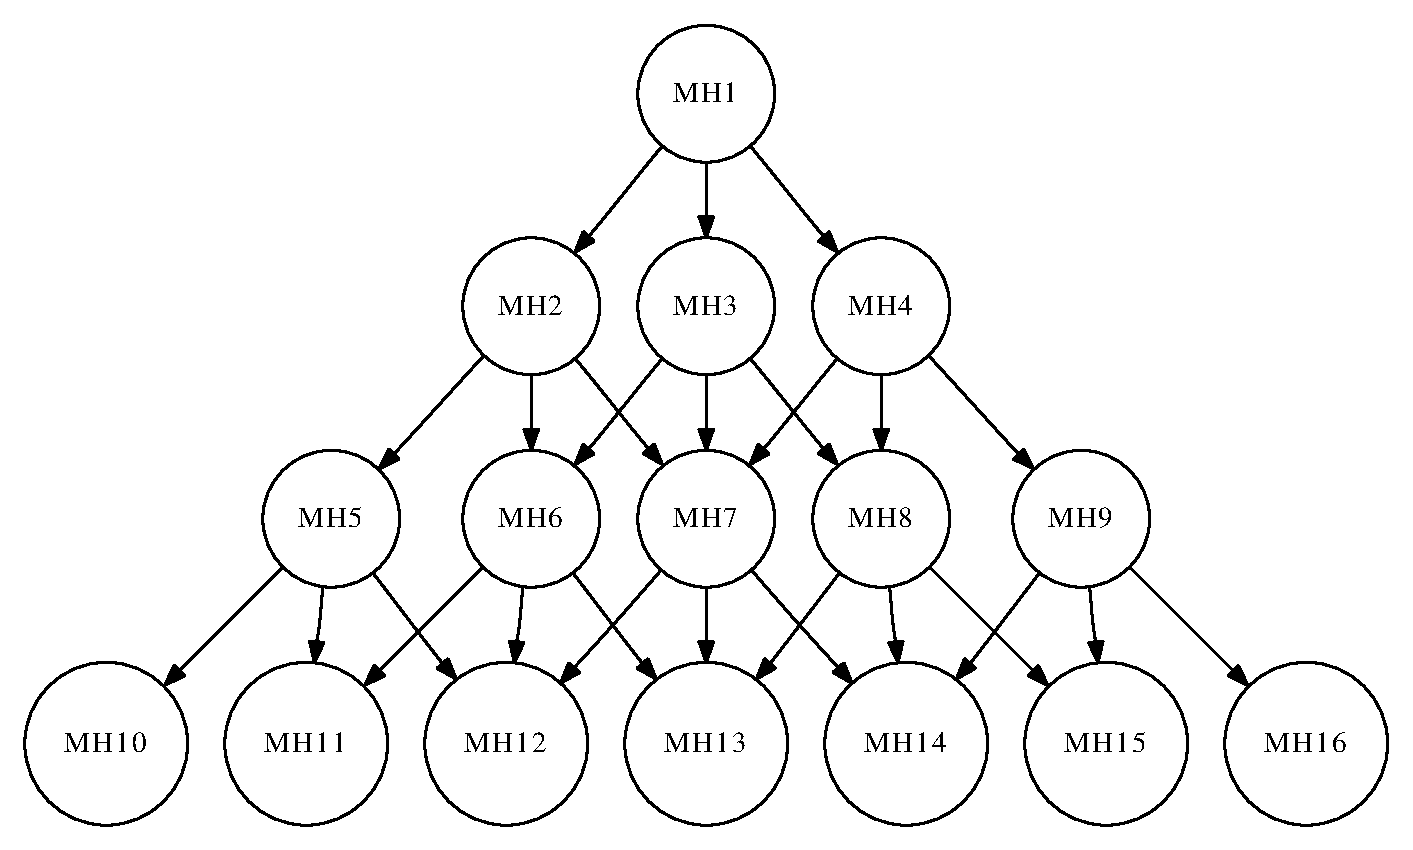
\includegraphics[scale=0.3]{olsrOperationStep4.eps}
	}\label{subfig:olsrStep14}	
	\caption{Descoberta de rotas de uma rede \textit{ad hoc} comum}
	\label{fig:olsrComum}
\end{figure}

\begin{figure}[H]
	\centering
	\subfigure[Primeiro est\'agio]{
		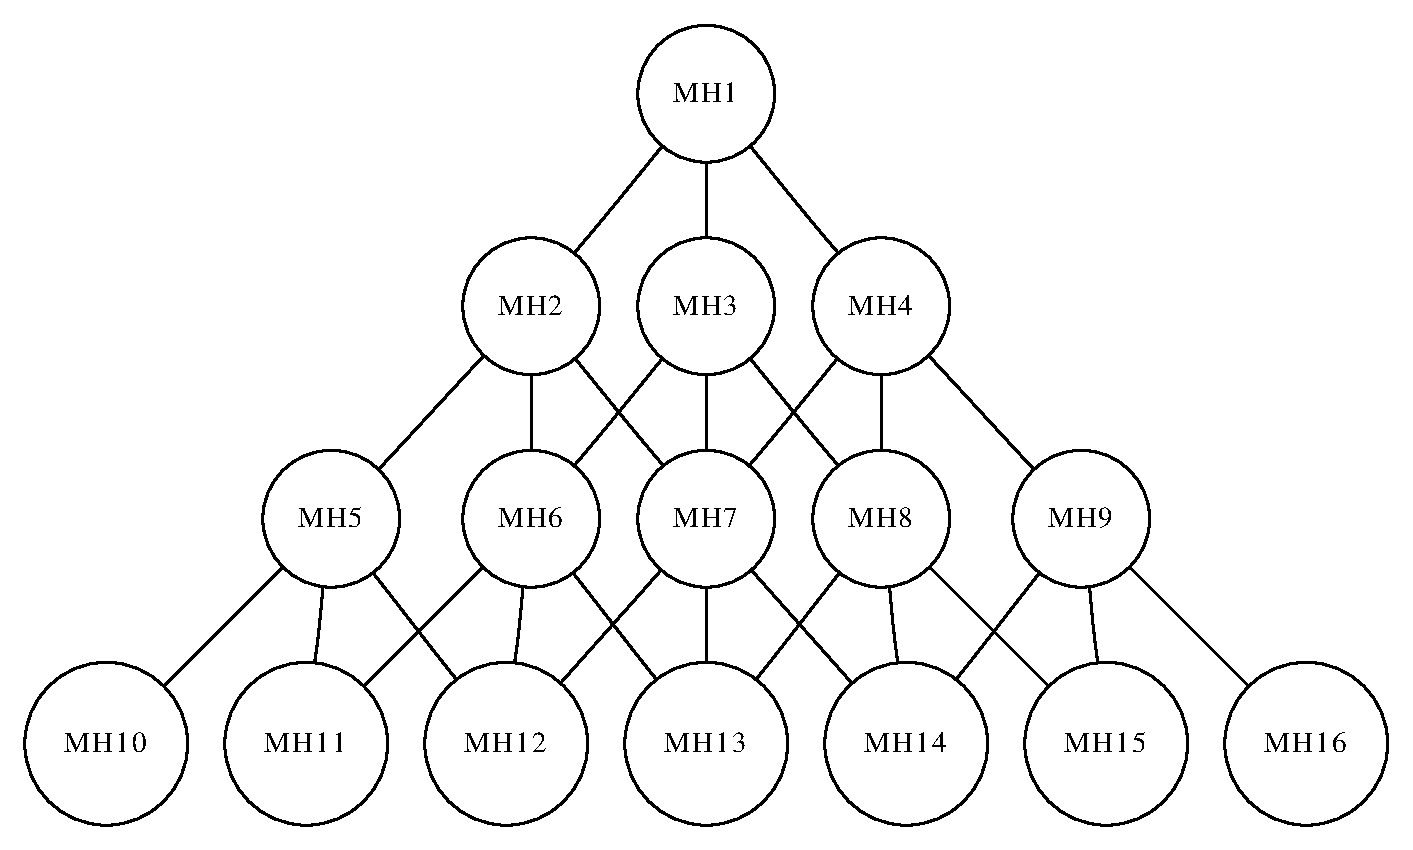
\includegraphics[scale=0.3]{olsrOperationStep1.eps}
	}\label{subfig:olsrStep21}
	\subfigure[Segundo est\'agio]{
		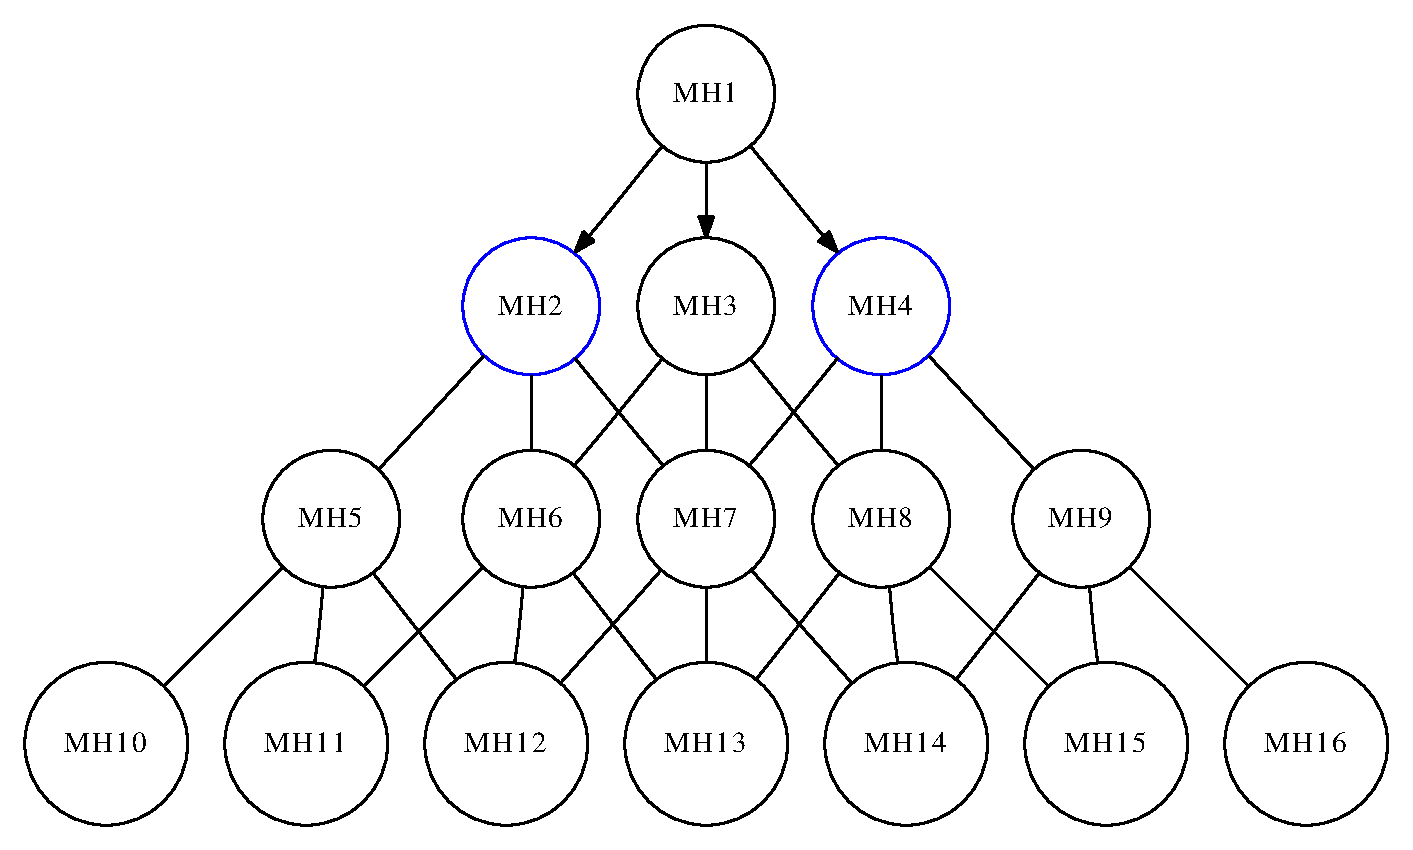
\includegraphics[scale=0.3]{olsrOperationStep5.eps}
	}\label{subfig:olsrStep22}
	\subfigure[Terceiro est\'agio]{
		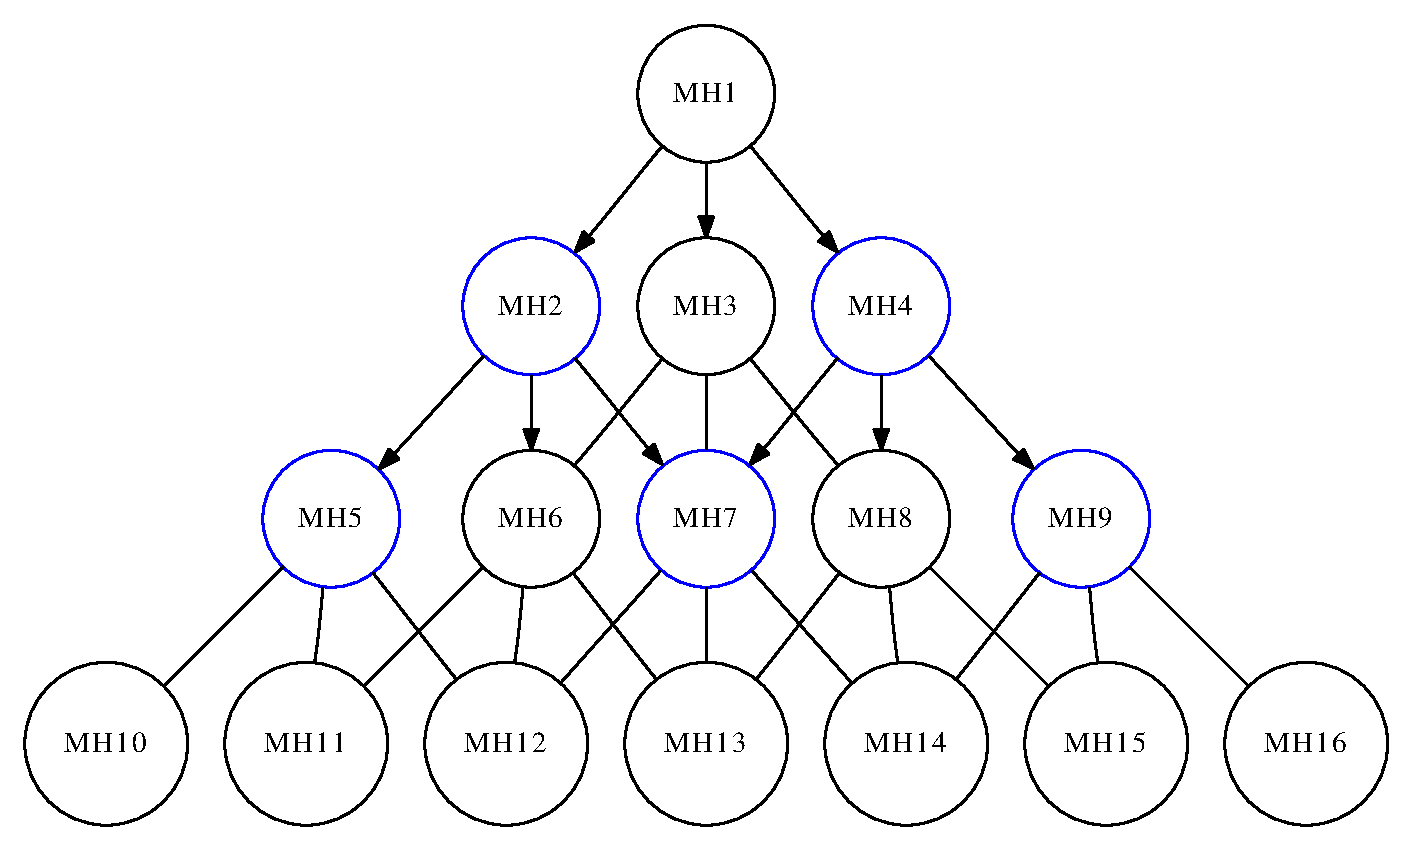
\includegraphics[scale=0.3]{olsrOperationStep6.eps}
	}\label{subfig:olsrStep23}
	\subfigure[Quarto est\'agio]{
		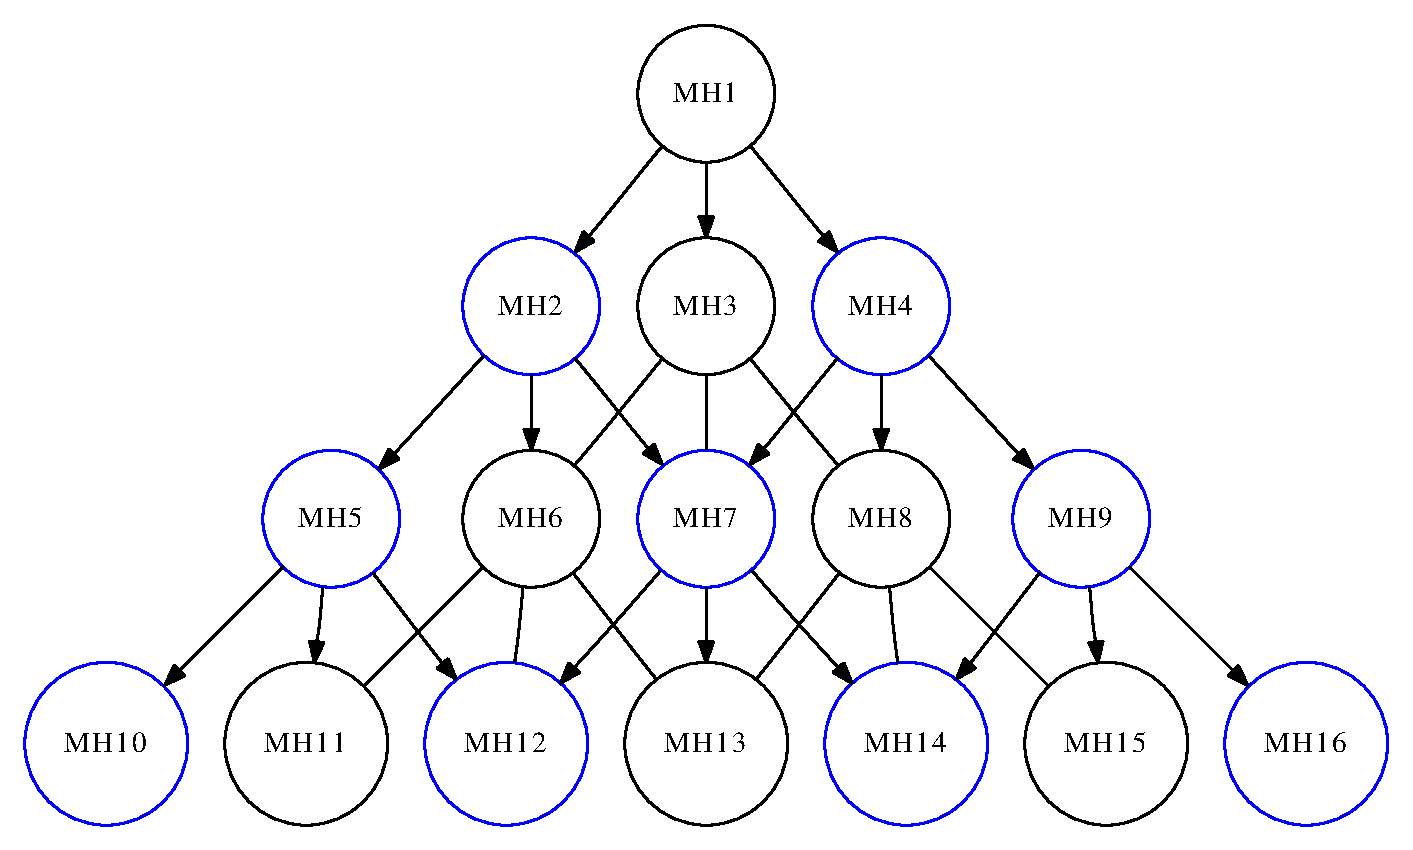
\includegraphics[scale=0.3]{olsrOperationStep7.eps}
	}\label{subfig:olsrStep24}	
	\caption{Descoberta de rotas do protocolo OLSR}
	\label{fig:olsrOperation}
\end{figure}
	%Optimized link state routing - OLSR
\subsection{Comparativo entre os protocolos} 
A tabela \ref{tabCompProt} demonstra um resumo de compara\c{c}\~oes analizadas entre os tr\^es procolos estudados nesse trabalho.

\begin{table}[H]
	\centering
	\caption{Caracter\'isticas entre os protocolos analizados}
	\begin{tabular}{ | l | l | l | }
		\hline
		Protocolo & Modo & Base \\ \hline
		DSDV & Pr\'o-ativo & Vetor de dist\^ancias \\ \hline
		AODV & Reativo & Vetor de dist\^ancias \\ \hline
		OLSR & Pr\'o-ativo & Estado de conex\~ao \\ \hline
	\end{tabular}
	\label{tabCompProt}
\end{table} %Comparação entre os protocolos
		%Protocolos de roteamento em redes ad hoc
\section{Metodologia dos testes} 

\subsection{Ambiente de simula\c{c}\~ ao}
Para o trabalho apresentado, os testes s\~ao baseados em simula\c{c}\~oes geradas pelo resultado de um projeto colaborativo entre a Universidade da Calif\'ornia do Sul e o laborat\'orio Xerox PARC, o simulador NS-2.

O NS-2 \'e um simulador de eventos discreto, oferecendo suporte \`a simula\c{c}\~ao de um grande n\'umero de topologias de redem duferentes cen\'arios baseados nos protocolos TCP e UDP, diversos escalonadores e pol\'iticas de fila, caracteriza\c{c}\~ao de tr\'afego com diversas distribui\c{c}\~oes estat\'isticas dentre outras finalidades.


\subsection{Cen\'arios militares}


	%Metodologia dos testes
\section{Experimentos e resultados}
\subsection{Experimentos}
Para compreender o funcionamento do simulador NS-2 e tamb\'em estudar simula\c{c}\~oes de comunica\c{c}\~ao em cen\'arios militares, foram definidos 2 experimentos te\'oricos, sendo o Experimento 1, um teste simples de converg\^encia de rotas, e o Experimento 2, baseado em estudos realizados por \cite{pereira}, o qual representa um caso de assalto e tomada de posi\c{c}\~ao inimiga.

Cada experimento possui suas caracter\'isticas, mas exite uma semalhan\c{c}a base, que \'e o tr\'afego que ir\'a caminhar pela rede, como comentado na se\c{c}\~ao \ref{trafegoDados}, o qual foi escolhido o CBR.

\subsubsection{Experimento 1}
O Experimento 1 baseia-se na ideia simples de um protocolo de rede \textit{ad hoc}, roteamento din\^amico.
O objetivo principal deste experimento \'e poder analisar o tempo de converg\^encia de roteamento de uma origem a um destino, alterando uma vez o caminho pelo qual eles realizam a comunica\c{c}\~ao.
A Tabela \ref{tabParamExp1} demonstra resumidamente os par\^ametros utilizados na execu\c{c}\~ao do Experimento 1.

\begin{table}[H]
	\centering
	\caption{Resumo dos par\^ametros usados no Experimento 1.}
	\begin{tabular}{ | l | l | }
		\hline
		N\'umero total de n\'os & 4 \\ \hline
		N\'umero de fontes de tr\'afego & 1 \\ \hline
		N\'umero de conex\~oes & 1 \\ \hline
		Tempo de simula\c{c}\~ao & 300 segundos \\ \hline
		\'Area total da simula\c{c}\~ao & 500x500 metros \\ \hline
		Tamanho dos pacotes & 512 \textit{bytes} \\ \hline	
		Velocidade dos n\'os & 1.5m/s constante \\ \hline
		Velocidade de banda & 11Mbps/s \\ \hline
	\end{tabular}
	\label{tabParamExp1}
\end{table}

A Figura \ref{figExp1} demonstra o experimento realizado, onde cada Soldado(n\'o) deve atingir seu respectivo Destino.
Cada Soldado inicia seu movimento a um tempo determinado na simula\c{c}\~ao, onde na Figura \ref{figExp1} \'e referenciado pelo prefixo \textit{at}, o qual \'e defido em segundos, e abaixo exibe o movimento de cada Soldado, onde nesse experimento todos os Soldados possuem um movimento constante de 1,5 metros por segundo. 

A fonte de tr\'afego nesse experimento \'e somente de uma, a qual realiza uma conex\~ao do Soldado 3(fonte) ao Soldado 1(destino). Inicialmente vai passar pelo Soldado 2 essa comunica\c{c}\~ao, pois os Soldados 1 e 3 n\~ao est\~ao pr\'oximos a fim de criarem uma rota direta.

\begin{figure}[H]
	\centering
	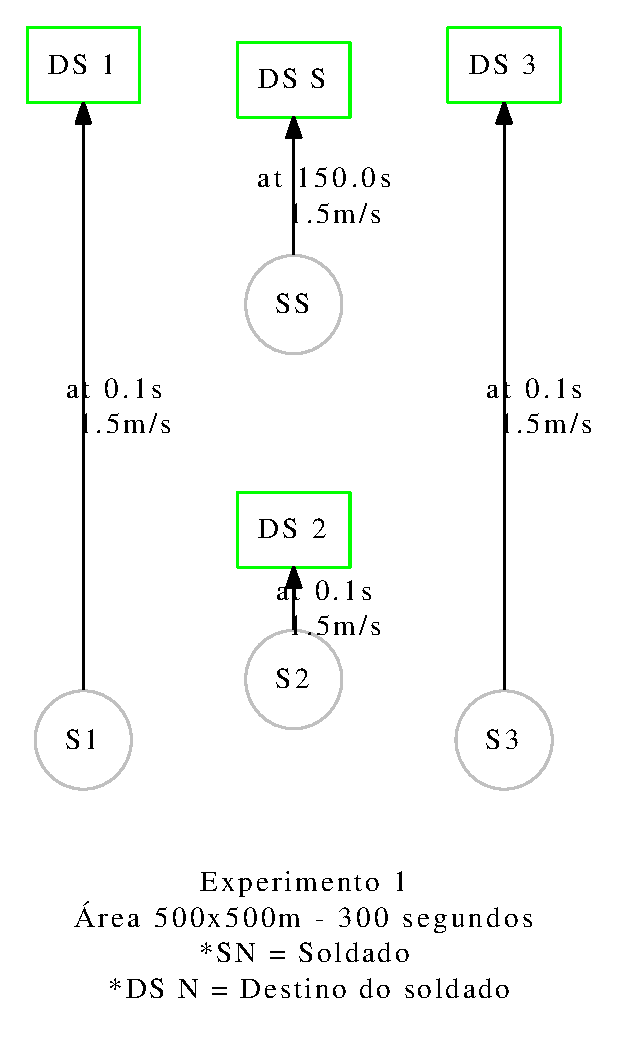
\includegraphics[scale=0.5]{experimento1.eps}
	\caption{Experimento 1}
	\label{figExp1}
\end{figure}

Observe que o Soldado 4 inicia somente seu movimento ao tempo de 150,0 segundos, enquanto os demais Soldados iniciam seus movimentos ao instante de 0,1 segundos.
Isso foi definido pelo fato do tempo em que o Soldado 2 atinja seu objetivo e pare de seguir em frente, enquanto os Soldados 1 e 3 continuam seus movimentos, e possam alcan\c{c}ar e estar dentro do raio de comunica\c{c}\~ao com o Soldado 4.
Quando os Soldados 1 e 3 se afastam do Soldado 2, eles perdem a sua rota por esse \textit{host} da rede, e necessitam buscar uma nova rota, a qual seguir\'a pelo Soldado 4, e \'e nesse ponto onde cada protocolo dever\'a gerar resultados distintos.

\subsubsection{Experimento 2}
O Experimento 2 foi baseado em estudos realizados por \cite{pereira} em sua tese de mestrado. 
O objetivo deste experimento \'e analisar o desempenho dos protocolos de roteamento como um todo em um cen\'ario militar. 
\cite{pereira} comenta que esse \'e um cen\'ario t\'ipico de simula\c{c}\~ao de uma opera\c{c}\~ao de assalto e tomada de posi\c{c}\~ao inimiga.

Esse cen\'ario consiste em 4 grupos de soldados e 1 ve\'iculo de apoio, e cada grupo de soldados \'e formado por 4 soldados.
Cada grupo possui um comandante, o qual envia ordens aos outros soldados do grupo, e tamb\'em recebe e envia ordens do ve\'iculo de apoio, este qual \'e encarregado de repassar as ordens aos demais grupos.
Cada grupo nesse cen\'ario tem como objetivo tomar a posi\c{c}\~ao inimiga, onde na Figura \ref{figExp2} est\'a descrito como "Destino final".

\begin{figure}[H]
	\centering
	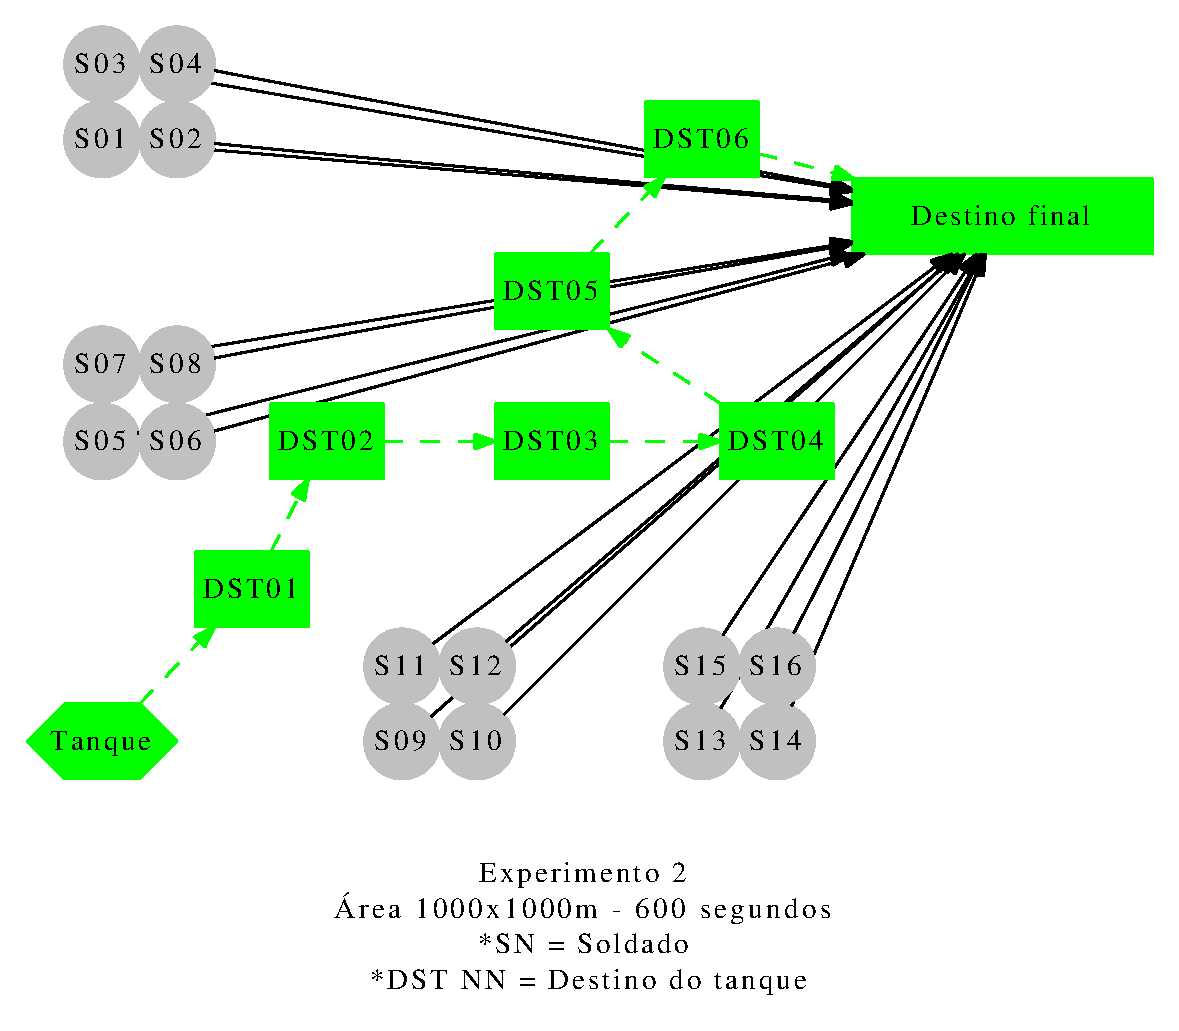
\includegraphics[scale=0.5]{experimento2.eps}
	\caption{Experimento 2}
	\label{figExp2}
\end{figure}

Todos os soldados de cada grupo dever\~ao avan\c{c}ar juntos durante o percurso do cen\'ario, n\~ao executando necessariamente um caminho reto durante todo o trajeto.

A Tabela \ref{tabParamExp2} demonstra resumidamente os par\^ametros utilizados nesse experimento. 
Al\'em do tamanho e n\'umero de conex\~oes e n\'os diferentes do Experimento 1, podemos verificar que a velocidade dos n\'os possuem uma varia\c{c}\~ao.
Essa varia\c{c}\~ao ocorre pelo fato de que, os soldados recebem ordens de parada ou avan\c{c}o no percurso, sendo que em cada situa\c{c}\~ao \'e necess\'ario aumentar, diminuir ou at\'e mesmo parar o ritmo de avan\c{c}o no objetivo do cen\'ario.

\begin{table}[H]
	\centering
	\caption{Resumo dos par\^ametros usados no Experimento 2.}
	\begin{tabular}{ | l | l | }
		\hline
		N\'umero total de n\'os & 17 \\ \hline
		N\'umero de fontes de tr\'afego & 7 \\ \hline
		N\'umero de conex\~oes & 16 \\ \hline
		Tempo de simula\c{c}\~ao & 600 segundos \\ \hline
		\'Area total da simula\c{c}\~ao & 1000x1000 metros \\ \hline
		Tamanho dos pacotes & 512 \textit{bytes} \\ \hline
		Velocidade dos n\'os & 0 \`a 8 m/s constante \\ \hline
		Velocidade de banda & 11Mbps/s \\ \hline
	\end{tabular}
	\label{tabParamExp2}
\end{table}

\subsection{An\'alise comparativa dos resultados}
As Figuras \ref{fig:resulExp1} e \ref{fig:resulExp2} apresentam atrav\'es de gr\'aficos os resultados obtidos dos experimentos executados. Esses resultados possibilitaram a formula\c{c}\~ao das conclus\~oes apresentadas mais adiante nesse trabalho.

\subsubsection{Experimento 1}
Nos gr\'aficos da Figura \ref{fig:resulExp1} \'e poss\'ivel notar que n\~ao houveram muitas diferen\c{c}as entre os dados dos diferentes protocolos. A ideia do experimento aqui apresentado \'e testar o tempo de converg\^encia, o qual nos gr\'aficos \'e representado pela Figura \ref{fig:resulExp1}(b).

Podemos perceber que a cada instante de tempo, temos pequenas diferen\c{c}as de roteamento, estes representados pelos gr\'aficos (c) e (d) da Figura \ref{fig:resulExp1}. A Tabela \ref{tabExp1Result} demonstra melhor estes resultados, sendo o resultado do total de dados trafegados pela rede no Experimento 1.

\begin{table}[H]
	\centering
	\caption{Resultado das simula\c{c}\~oes do Experimento 1}
	\begin{tabular}{ | c | c | c | c | }
		\hline
		M\'ETRICAS AVALIADAS & DSDV & AODV & OLSR \\ \hline
		Taxa de entrega & 92.98\% & 99.83\% & 98.43\% \\ \hline
		Atraso m\'edio (ms) & 10.7575 & 11.4837 & 11.3047 \\ \hline
		N\'umero de pacotes & 543 & 588 & 565 \\ \hline
		N\'umero de \textit{bytes} & 288896 & 312816 & 300580 \\ \hline
	\end{tabular}
	\label{tabExp1Result}
\end{table}

Podemos analisar que o DSDV obt\'em uma r\'apida vantagem em n\'umero de pacotes e \textit{bytes} gerados no experimento em rela\c{c}\~ao aos demais protocolos. Por\'em essa r\'apida vantagem \'e anulada pela taxa de entrega, que foi bem menor em rela\c{c}\~ao ao protocolo AODV e OLSR.

O objetivo inicial desse experimento era analisar o tempo de converg\^encia entre os protocolos, o qual n\~ao foi muito significativo, pois resultou em diferen\c{c}as menores de 1 ms entre os protocolos de roteamento. 
O destaque nesse experimento ficou na taxa de entrega, pois demonstra que o OLSR e o AODV mantiveram uma taxa pr\'oximo de 100\%, e o DSDV obteve uma taxa inferior.

\subsubsection{Experimento 2}
Diferentemente do Experimento 1, o Experimento 2 possui caracter\'isticas diferentes de mobilidade, onde cada soldado no cen\'ario n\~ao vai percorrer um caminho cont\'inuo e tamb\'em n\~ao vai ter uma velocidade constante de avan\c{c}o para o objetivo final do cen\'ario.
A fim de trazer uma m\'edia de resultados satisfat\'orios, foram gerados e executados simula\c{c}\~oes de cen\'arios 15 vezes, a fim de obter uma m\'edia somat\'oria entre os dados.
Os gr\'aficos da Figura \ref{fig:resulExp2} demonstram os resultados obtidos no experimento 2.

Com rela\c{c}\~ao as Figuras \ref{fig:resulExp2}(c) e \ref{fig:resulExp2}(d), o comportamento \'e similar, pois como cada pacote tem um tamanho fixo de 512 \textit{bytes}, o n\'umero de \textit{bytes} de roteamento vai ser proporcional ao n\'umero de pacotes de roteamento.

Em rela\c{c}\~ao a m\'etrica de Taxa de Entrega, podemos notar que h\'a pequenas oscila\c{c}\~oes, e que somente o protocolos AODV teve uma grande perda de informa\c{c}\~oes.

\begin{table}[H]
	\centering
	\caption{Resultado das simula\c{c}\~oes do experimento 2}
	\begin{tabular}{ | c | c | c | c | }
		\hline
		M\'ETRICAS AVALIADAS & DSDV & AODV & OLSR \\ \hline
		Taxa de entrega & 96.88\% & 90.37\% & 95.29\%  \\ \hline
		Atraso m\'edio(ms) & 8.15969 & 16.3527 & 6.88545  \\ \hline
		N\'umero de pacotes & 7407 & 7696 & 7483  \\ \hline
		N\'umero de \textit{MegaBytes} & 3.76 & 3.90 & 3.80  \\ \hline
	\end{tabular}
	\label{tabExp2Result}
\end{table}

A Tabela \ref{tabExp2Result} demonstra um resultado total do Experimento 2. Nela podemos avaliar que o AODV teve um desempenho inferior no desempenho de entrega dos pacotes, que pode ser conferido na Figura \ref{fig:resulExp2}(b), gerou mais pacotes e teve uma taxa de entrega inferior.
	%Experimentos e resultados
\section{Conclus\~ao e trabalhos futuros}\label{conclusao}

As simula\c{c}\~oes apresentadas neste trabalho confirmam o fato de que cada protocolo apresenta vantagens e desvantagens, dependendo das condi\c{c}\~oes que lhe s\~ao impostas, como no caso, o n\'umero de n\'os na rede. 
Nos cen\'arios com prop\'ositos militares, que utilizam redes \textit{ad hoc} com configura\c{c}\~ao hier\'arquica, a entrega dos pacotes de forma eficiente e r\'apida \'e de extrema relev\^ancia. 
O protocolo "ideal"\ atenderia a todas as restri\c{c}\~oes impostas pelas necessidades de comunica\c{c}\~ao em cen\'arios tipicamente militares, mas o que se p\^ode concluir, a partir dos resultados alcan\c{c}ados, \'e que cada um dos protocolos avaliados mostrou sua diferen\c{c}a em determinada m\'etrica ou condi\c{c}\~ao.

Entre os protocolos analisados, pode ser observado que o DSDV e o AODV tiveram comportamentos opostos nos dois experimentos realizados, e que o OLSR manteve uma boa estabilidade entre ambos os experimentos.

Para futuras pesquisas, sugere-se que seja combinada algumas caracter\'isticas de protocolos, prevalecendo das situa\c{c}\~oes em que eles apresentam maiores vantagens nos cen\'arios propostos.
Bem como, sugere-se que sejam testados outros protocolos e mudan\c{c}as de cen\'arios.
Aos interessados em continuar o desenvolvimento desse trabalho, ou ent\~ao reproduzir os experimentos, \'e poss\'ivel obter todos os cen\'arios, \textit{script} de extra\c{c}\~ao dos dados, e a vers\~ao deste artigo em latex, acessando o link dispon\'ivel em \cite{fabiosammy}.
		%Conclusão

%Referencias bibliograficas sao editadas no arquivo referencias/bibliografias.bib
\newpage
\section{Refer\^encias bibliogr\'aficas}
%\bibliographystyle{sbc}
\bibliographystyle{abnt-alf}
\def\bibindent{0.5cm}
\renewcommand{\emph}{\textbf}
\bibliography{referencias}

\end{document}
